\section{Visualizations of Dataset}
\begin{fullwidth}First, it is important to analyze and visualize the properties of the original images. 
We did this with the following steps\dots\end{fullwidth}

\subsection{BGR channels of original dataset}
\sidenote{We needed to analyze the color distribution of the colors to understand the average colors used within the dataset. 
The figure below shows the result of this analysis for the whole dataset and below that examples of 3 random images and their own color channels.}

\begin{figure}[H] % [H] forces the figure to be output where it is defined in the code (it suppresses floating)
	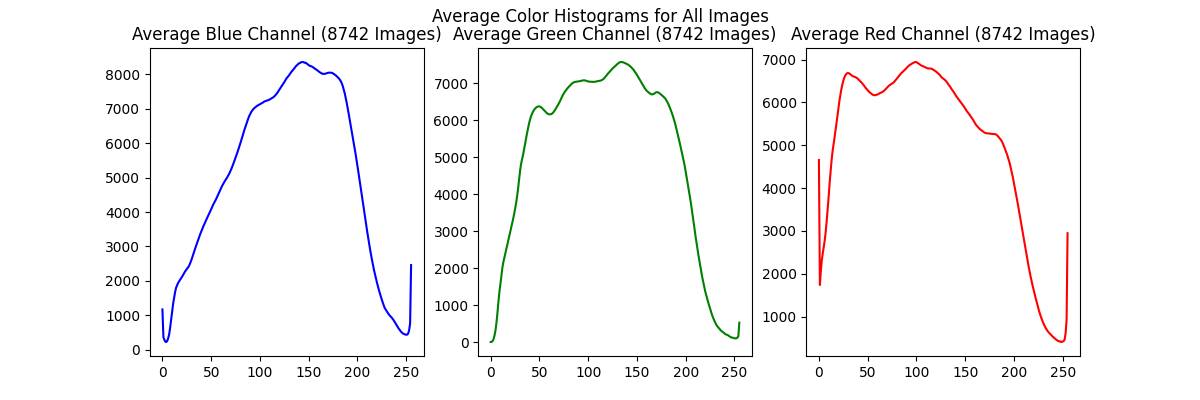
\includegraphics[width=\linewidth]{average_color_histogram.png}
	\caption{Average colourchannels}
	\label{fig:average_color_histogram} % Label for referencing this figure in the text automatically
\end{figure}

\begin{figure}[H] % [H] forces the figure to be output where it is defined in the code (it suppresses floating)
	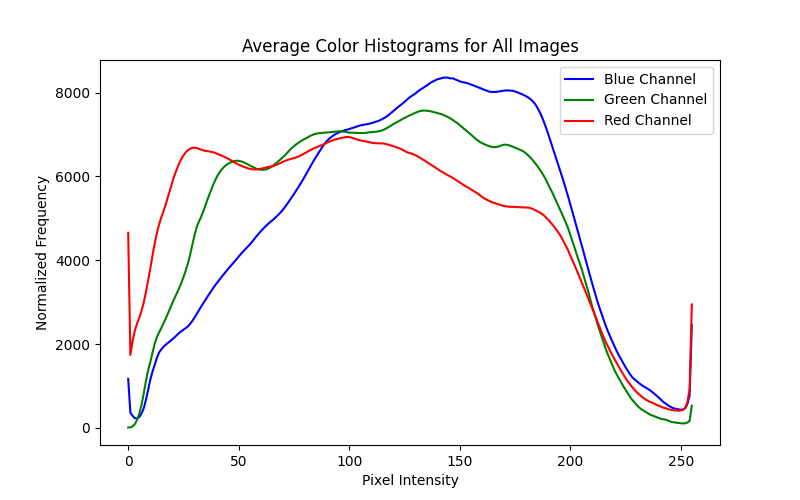
\includegraphics[width=\linewidth]{average_color_histogram_overlap_full.png}
	\caption{Overlapping average colourchannels}
	\label{fig:average_color_histogram_overlap_full} % Label for referencing this figure in the text automatically
\end{figure}

\newpage
\subsection{Visualizing aspect ratios}
\sidenote[][]{We also need to check the aspect ratios to check whether non-square images were present in our dataset. And as you can see, not all have a square aspect ratio. However, this is required for most and simpler YOLO algorithms}

\begin{figure}[H] % [H] forces the figure to be output where it is defined in the code (it suppresses floating)
	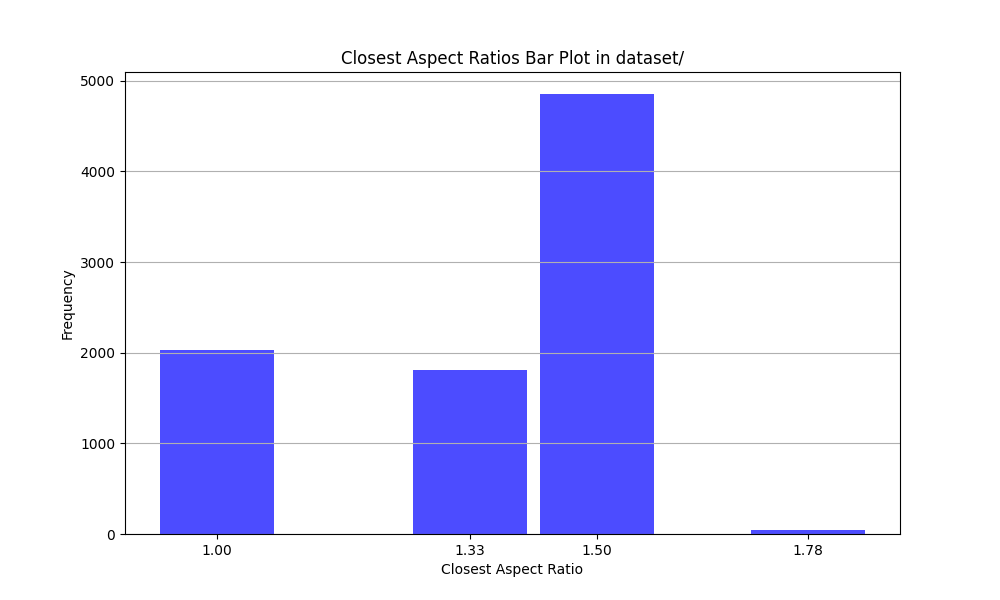
\includegraphics[width=\linewidth]{aspect_ratio_result.png}
	\caption{Aspect ratios}
	\label{fig:aspect_ratio_result} % Label for referencing this figure in the text automatically
\end{figure}

\newpage
\subsection{Visualizing resolutions}
\begin{fullwidth} % Use the whole page width
Before changing the properties of the images, 
we also need to check the resolutions to determine if we can safely decrease it to make it easier to work with the model without long loading times which comes with using big files. 
All images in the dataset we got from the client had roughly had a 4K resolution, which meant each image was around 4- to 6MB in size. 
This meant the total dataset was around 75GB for 7800 images. 
The size means that the dataset is difficult to process in code and the model generally does not require images with a resolution that large. 
We decided to scale the images down when the resolution was of a higher value than 3000 in either width or length. 
This meant a file size decrease of about 94\%. 
This resulted in the total size of the dataset decreasing to less than 4GB and thus being much easier to process. 
The figure below shows the result resolution rescaling.
\end{fullwidth} % End of use the whole page width

\sidenote{Rescaling was done immediatly since the 8742 images within the dataset resulted in a size of over 75GB which isn't easy to work with.}
\begin{figure}[H] % [H] forces the figure to be output where it is defined in the code (it suppresses floating)
	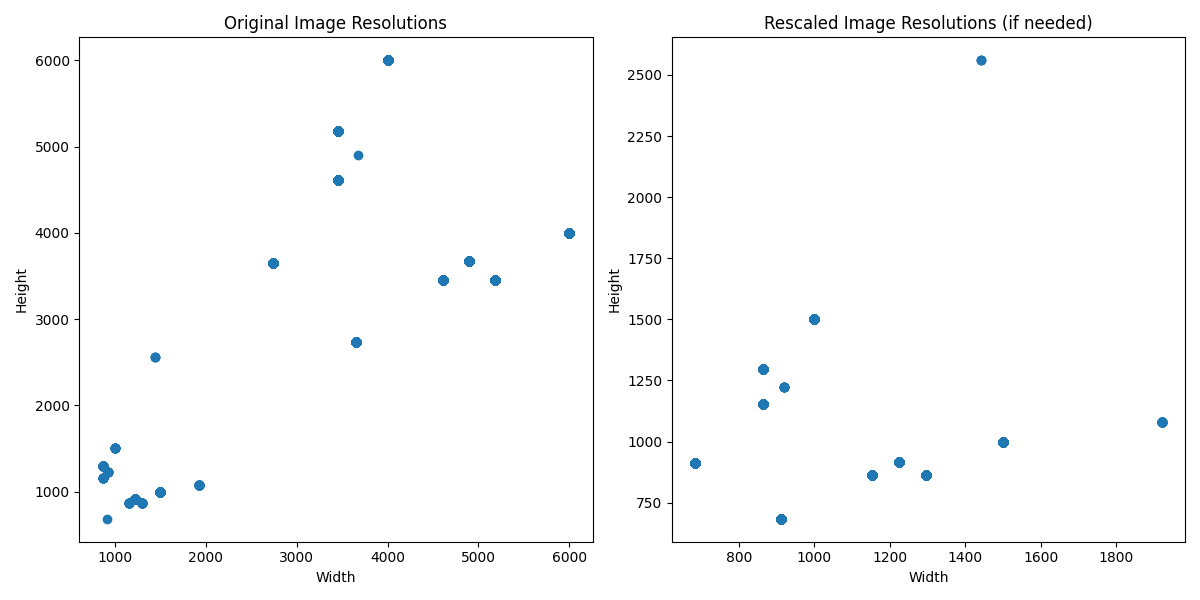
\includegraphics[width=\linewidth]{rescale_res_result.png}
	\caption{Resolutions of images before \& after}
	\label{fig:rescale_res_result} % Label for referencing this figure in the text automatically
\end{figure}

% \begin{marginfigure} % Use the marginfigure environment for figures to be output to the margin
% 	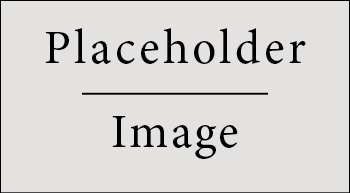
\includegraphics[width=\linewidth]{placeholder.jpg}
% 	\caption{Margin figure caption.}
% \end{marginfigure}

% \begin{marginfigure} % Use the marginfigure environment for figures to be output to the margin
% 	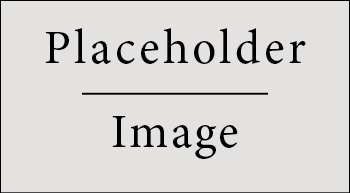
\includegraphics[width=\linewidth]{placeholder.jpg}
% 	\caption{Margin figure caption.}
% \end{marginfigure}